% vim: spell spelllang=en:
%! TEX root = **/00-main.tex


% Formal description of Data structure and metadata

\section{Description of data}%
\label{sec:description_of_data}

\subsection{Description of initial data matrix}

The data set has 20,703 entries and 74 variables, out of which 30 are categorical,
38 are numerical and 6 are boolean, meaning that there are 1,532,022 data entries.
The share of missing data is 9.01\%, or 138,007
entries in absolute terms. We should note that two variables, \texttt{bathrooms} and
\texttt{calendar\_updated}, have NA values for all records and hence are useless. 
If we remove those two variables, the share of missing data drops to 
around 6.5\%.
Furthermore, for a few variables such as \texttt{neighbourhood} and all variables
related to reviews we have a significant share of NA entries, around 25 and 30\%
or 5,000 to 7,000 in absolute terms. The rest of the variables have largely no 
missing data and the few that do are below 3\%.

Regarding the hosts, it tells us about, among other things, when they joined
\airbnb, where they live, how long they take to respond 
messages, their acceptance and response rates, whether they are superhosts, how 
many listings they have or whether they have a profile picture.

The information it supplies concerning the listings includes its
neighbourhood, its coordinates, the type of property it is, the number of people 
it accommodates, the number of bedrooms, beds and bathrooms, amenities, price, 
the minimum and maximum nights it can be rented, its availability and reviews.

Additionally, the data set contains variables that don't provide useful information 
such as URLs, identifications numbers, names and descriptions or some dates.

% TODO
% What do rows of data matrix contain? (one paragraph)

% Metadata Table

% TODO - Recompilar metadata
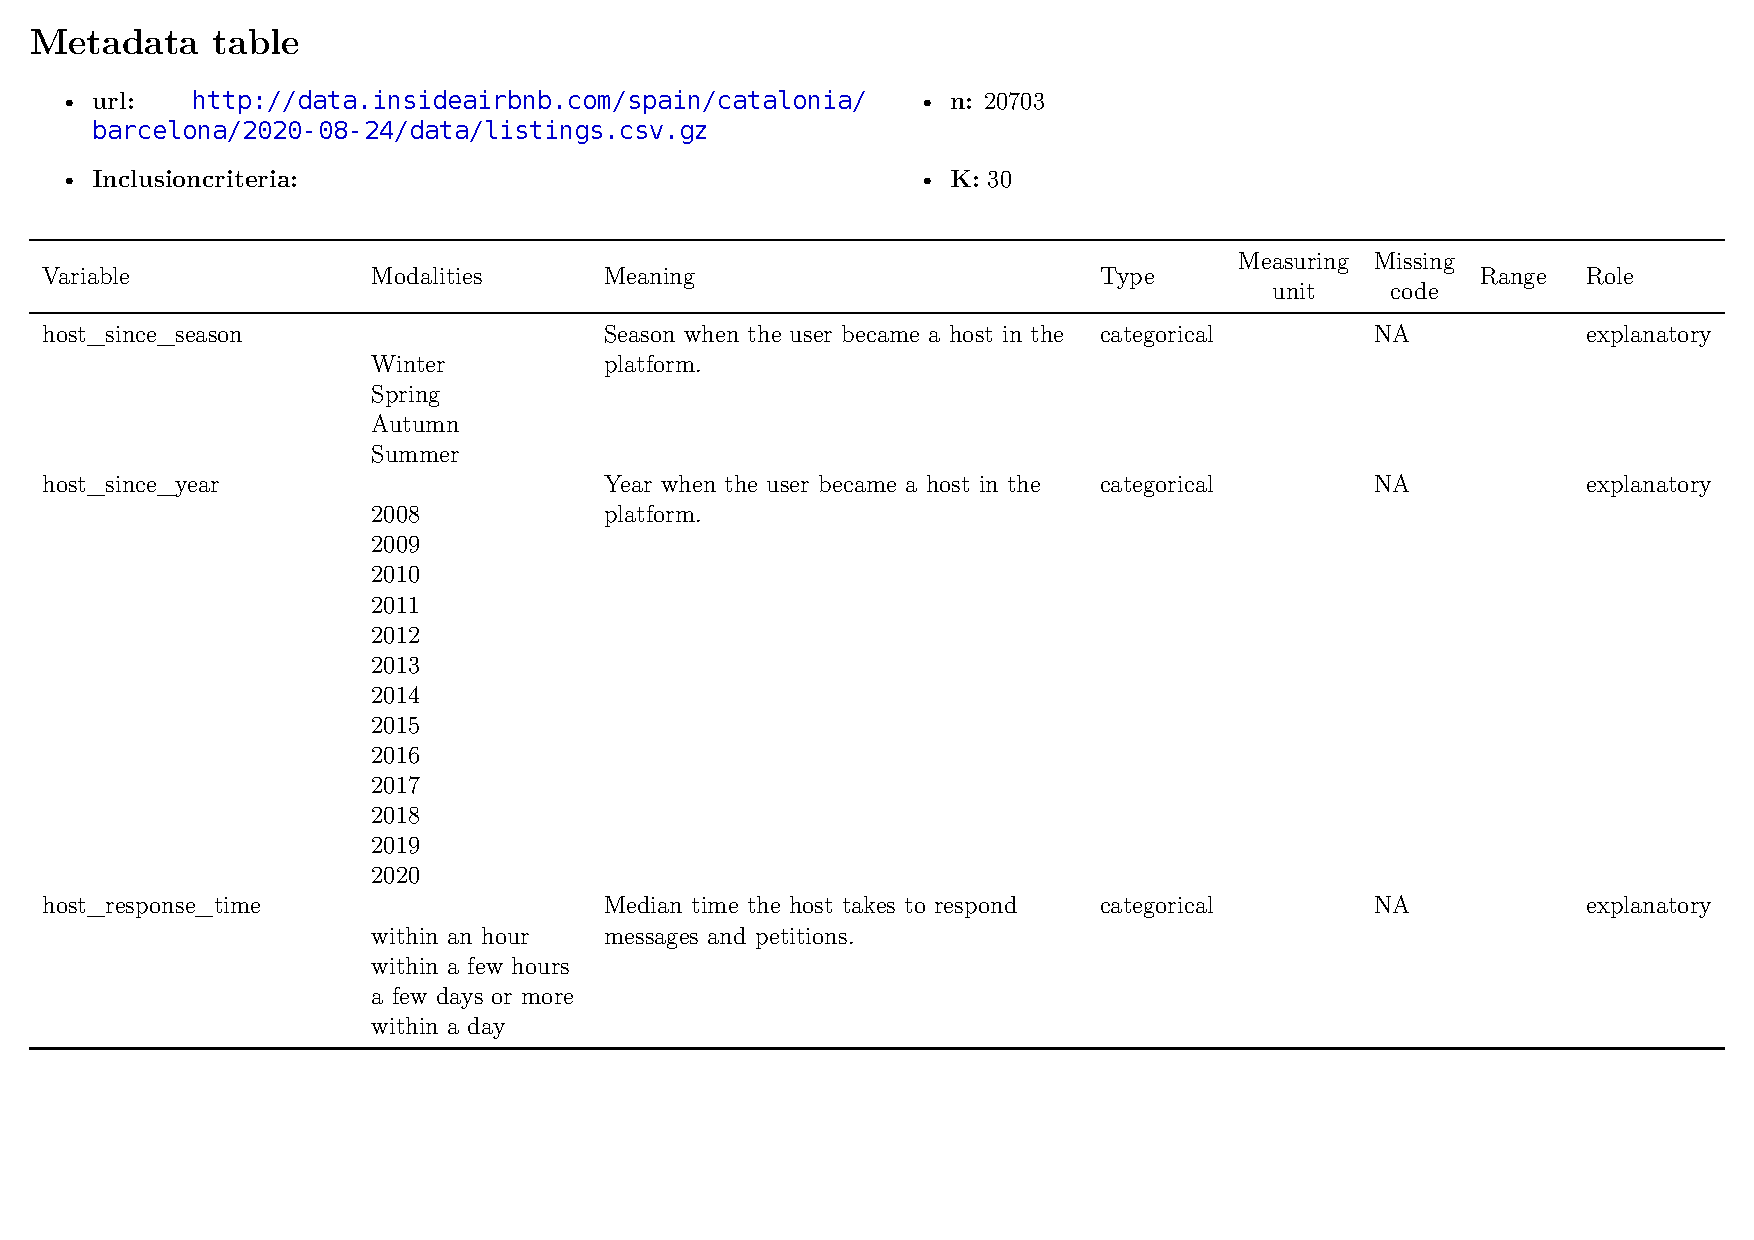
\includepdf[pages=-,landscape=true]{../metadata_table/metadata}



% TODO
% Final scope of the study with inclusion and exclusion criteria for both rows
% and columns (max half a page)
\subsection{Final scope of study}

After considering what variables were appropriate for our study, we decided to keep 
those shown in the metadata table presented above. We chose these because
we believe they provide real insight into the question we are posing in this study,
in which we aim to find what factors affect most the obtention of positive reviews
and high ratings. Those are variables that describe the nature of the host or
the listing in an abstract manner, allowing us to analyze the listings adequately.

We discarded the rest
of the variables during preprocessing, either because they were duplicated or
irrelevant. Furthermore, we extrapolated a few variables and created 
two new ones, this process is explained in higher detail in the preprocessing 
section. This resulted in a cleansed data set that contains 30 variables: 
20 numerical, 7 categorical and 4 boolean.